\documentclass[12pt]{article}
\usepackage[utf8]{inputenc}
\usepackage[T2A]{fontenc}
\usepackage[english,russian]{babel}
\usepackage{alltt}
\usepackage{amsfonts}
\ifx\pdfoutput\undefined
\usepackage{graphicx}
\else
\usepackage[pdftex]{graphicx}
\fi
\usepackage{amssymb}
\usepackage{amsmath}
\usepackage{mathtext}
\usepackage{parskip}
\usepackage[left=2cm,right=2cm,
    top=2cm,bottom=2cm,bindingoffset=0cm]{geometry}
\renewcommand{\contentsname}{ОГЛАВЛЕНИЕ}
	
\begin{document}

\begin{titlepage}
\large
\begin{center}
ФЕДЕРАЛЬНОЕ ГОСУДАРСТВЕННОЕ БЮДЖЕТНОЕ\\ ОБРАЗОВАТЕЛЬНОЕ УЧРЕЖДЕНИЕ ВЫСШЕГО ОБРАЗОВАНИЯ \\ <<МОСКОВСКИЙ ГОСУДАРСТВЕННЫЙ УНИВЕРСИТЕТ \\ имени М.В.ЛОМОНОСОВА>>  
\end{center}
\begin{center}
МЕХАНИКО-МАТЕМАТИЧЕСКИЙ ФАКУЛЬТЕТ
\end{center}
\begin{center}
КАФЕДРА ТЕОРИИ ВЕРОЯТНОСТЕЙ
\end{center}
\parskip=50pt 
\begin{center}
ВЫПУСКНАЯ КВАЛИФИКАЦИОННАЯ РАБОТА \\
(ДИПЛОМНАЯ РАБОТА)\\
специалиста
\end{center}
\parskip=20pt 
\begin{center}
СИСТЕМЫ ОБСЛУЖИВАНИЯ С ПЕРЕРЫВАМИ \\
В РАБОТЕ ПРИБОРА И ЗАДЕРЖКАМИ
\end{center}
\parskip=60pt 
\begin{flushleft}
\leftskip=9cm \rightskip=0cm
Выполнила студентка\\
631 группы \\
Рассохина Александра Николаевна
\end{flushleft}
\parskip=25pt
\begin{flushleft}
\leftskip=9cm \rightskip=0cm
\underline{\hspace{4cm}}\\
подпись студента
\end{flushleft}
\parskip=10pt
\begin{flushleft}
\leftskip=9cm \rightskip=0cm
Научный руководитель:\\
д. ф.-м.н., профессор \\Афанасьева Лариса Григорьевна
\end{flushleft}
\parskip=25pt
\begin{flushleft}
\leftskip=9cm \rightskip=0cm
\underline{\hspace{4cm}}\\
подпись научного руководителя
\end{flushleft}
\vspace{1.3cm}
\begin{center}
Москва\\
2021
\end{center}
\end{titlepage}

\renewcommand{\contentsname}{Оглавление}
\tableofcontents
\newpage
\section{Введение}
Исследование систем обслуживания, в которых прибор на случайное время становится полностью или частично недоступным, началось c семидесятых годов прошлого века, с тех пор, как идея перерывов впервые обсуждалась в работе $[2]$. \\
\\
Для такой частичной или полной временной недоступности прибора в англоязычной литературе существует термин \textit{vacation}. В литературе на русском языке общепринятого термина нет. В нашей работе мы используем выражение $"$перерыв в работе прибора$"$, считая, что перерывы могут начинаться в моменты, когда в системе нет требований. Существует множество систем с разными правилами поведения в течение перерыва: полное отключение, обслуживание требования другим, например, менее эффективным прибором и прочие. В нашей работе мы рассматриваем перерыв как полное отключение прибора, однако, учитываем возможность обрыва перерыва, когда в системе скопилось слишком большое число требований. Требования, поступившие в систему во время перерыва начинают обслуживаться только по завершении перерыва.\\
\\
В некоторых системах до принятия решения о перерыве проходит случайное время, которое мы будем называть задержкой. Требования, поступающие в систему во время задержки, поступают на обслуживание сразу же. Система, в которой присуствуют и задержки, и перерывы, также будет рассмотрена в нашей работе.\\
\\
Системы обслуживания с перерывами и задержками используются для моделирования многих процессов. Перерыв в обслуживании может быть следствием многих факторов. Например, он может быть вызван необходимостью профилактического осмотра или ремонта оборудования, или же необходимостью использовать прибор в других, более загруженных системах, чтобы избежать длительных простоев и неэффективного использования оборудования. \\
\\
В нашей работе мы рассмотрим две модели. В первой модели рассматривается перерыв, который обрывается, когда в системе скапливается $m$ требований. Во второй в моменты освобождения системы от требований начинается период задержки, и, если во время задержки требований так и не поступило, с вероятностью $\alpha$ прибор переходит в перерыв, то есть обслуживание прекращается на некоторое случайное время. Обе модели одноканальные с пуассоновским входящим потоком и экспоненциально распределенными временами перерывов и задержек. Времена обслуживания одной заявки прибором также имеют экспоненциальное распределение.\\
\\
Далее мы подробнее остановимся на каждой из двух моделей и найдем формулы для распределения и математического числа требований в системе в стационарном режиме. Также мы приведем оптимизацонную задачу, в которой исследуется оптимальное число заявок, при которых следует выводить прибор из перерыва, чтобы минимизировать издержки, обусловленные, с одной стороны, простоем прибора, с другой -- ожиданием обслуживания требованиями, пришедшими в систему.
\\ 
\section{Модель с перерывами в работе прибора}
\subsection{Описание модели}
Рассмотрим одноканальную систему с перерывами в обслуживании, но без задержек. Все требования, пришедшие за время перерыва обслуживаются прибором только по окончании перерыва. То есть во время перерыва обслуживания нет. Пусть входящий поток -- пуассоновский с параметром $\lambda$, $\eta$ -- длительность перерыва, случайная величина, экпоненциально распределенная с параметром $\nu$. Времена обслуживания прибора распределены экспоненциально с параметром $\mu$.\\
В этой модели рассматривается перерыв, который обрывается, когда в системе скапливается $m$ требований. Устремив $m$ к бесконечности, мы получаем систему, в которой обрываться не будет.\\
\\
$Y(\eta)$ -- количество заявок, пришедших за перерыв длительности $\eta$, $t_m$ -- момент прихода m-го требования, $t_m \in (t, t+\eta)$. Мы рассмотрим случай, когда при приходе $m$ требований перерыв оборваетcя, и начинается обслуживание, значит, введем обозначения, учитывающие обрыв перерыва.\\
\\
$\tilde{Y}(\eta)$ -- количество заявок, пришедших в систему, с учетом обрыва перерыва.\\
$\tilde{\eta}$ -- длительность перерыва, с учетом того, что он может оборваться.\\
\\
Выразим случайные величины $\tilde{Y}(\eta)$ и $\tilde{\eta}$ через $Y(\eta)$ и $\eta$:
$$ (\tilde{Y}(\eta), \tilde{\eta}) = (Y(\eta), \eta)\cdot\mathbb{I}(Y(\eta) < m) + (m, t_m)\cdot\mathbb{I}(Y(\eta) \geqslant m). $$
Определим функции
$$G(z,s) = \mathbb{E}z^{Y(\eta)}e^{-s\eta}, \hspace{1.5cm} g(s) = G(1,s), $$
$$C(z) = \mathbb{E}z^{Y(\eta)} = G(z,0) = \sum\limits^\infty_{j=0}C_jz^j, \hspace{1cm} |z| \leqslant 1, Re s \geqslant 0.$$
$$V(z,t) = \mathbb{E}z^{Y(t)}\mathbb{I}(\eta > t) = \sum\limits^{\infty}_{j=0}z^j\mathbb{P}(Y(t)=j, \eta > t). $$
Эти формулы нужны для нахождения распределения и математического числа требований в системе в стационарном режиме.\\ 
\\
Рассмотрим случайный процесс $q(t)$, представляющий собой число требований в нашей системе в момент $t$. Процесс $q(t)$ стабилен, если при любом начальном состоянии $q(0)$ существуют пределы
$$\lim_{t\to\infty} \textbf{P}(q(t) = j) = p_j, \hspace{1cm} (j = 0, 1, 2 ...), \hspace{1cm} \sum\limits^{\infty}_{j=0} p_j = 1, $$ 
не зависящие от начального состояния. Для цепи Маркова -- это свойство эргодичности.\\
\\
Процесс $q(t)$ -- регенерирующий, и в качестве его точек регенерации возьмем последовательные моменты $\{T_n\}^\infty_{n=1}$ возникновений перерывов, тогда, по теореме из работы [1], предполагая, что $\mathbb{E}\eta < \infty$ и $\textbf{P}(Y(\eta) = 0) < 1$, процесс $q(t)$ стабилен тогда и только тогда, когда $\rho = \dfrac{\lambda}{\mu} < 1.$
\subsection{Нахождение формулы предельного распределения процесса $\textbf{\textit{q(t)}}$}
Используя результат из работы [1], полученный для одноканальной системы с перерывами, но не учитывающий возможность обрыва перерывов, найдем предельное распределение для процесса $q(t)$.
\\
Если $\mathbb{E}\tilde{\eta} < \infty$ и $\rho < 1$, то существует 
$$\lim_{t\to\infty} \mathbb{E}z^{q(t)} = \pi(z) = \dfrac{1-\rho}{\lambda\bar{\eta}(1-\rho) + \rho Y_1}\times \left(\lambda\int\limits^\infty_0 \tilde{V}(z, t)\,dt + \dfrac{z(1-\tilde C(z))}{1-z} \cdot \dfrac{1-\beta(\lambda-\lambda z)}{\beta(\lambda-\lambda z) - z}\right), \eqno(1) $$
где $\beta(s) = \int\limits^\infty_0 e^{-sx}\, dB(x) = \int\limits^\infty_0 \mu e^{-(s+\mu)x}\, dx,  Y_1 = \mathbb{E}\tilde{Y}(\mu), \bar{\mu} = \mathbb{E}\tilde \mu.$\\
\\
Заметим, что для получения предельного распределения в нашей системе мы используем $\tilde{\eta}, \tilde{C(z)}, \tilde{V(z, t)}, \tilde{G(z, s)}$, которые получены из функций, введенных в 2.1, с учетом обрыва перерыва, то есть:
$$\tilde G(z,s) = \mathbb{E}z^{\tilde Y(\eta)}e^{-s\eta}, \hspace{1.5cm} \tilde g(s) = \tilde G(1,s), $$
$$\tilde C(z) = \mathbb{E}z^{\tilde Y(\eta)} = \tilde G(z,0), \hspace{1cm} |z| \leqslant 1, Re s \geqslant 0.$$
$$\tilde V(z,t) = \mathbb{E}z^{\tilde{Y}(t)}\mathbb{I}(\tilde{\eta} > t) = \sum\limits^{\infty}_{j=0}z^j\mathbb{P}(Y(t)=j, \tilde{\eta} > t). $$
\\
Найдём формулу для $\tilde{G}(z,s)$, а далее используем её вычисления других функций, использованных в формуле (1).\\
$$\tilde{G}(z,s) =\mathbb{E}z^{\tilde{Y}(\eta)}e^{-s\tilde{\eta}} = \sum\limits^{m-1}_{j=0}z^j\int\limits^\infty_0 e^{-sx}e^{-\lambda x} \dfrac{(\lambda x)^j}{j!} \nu e^{-\nu x}\, dx + z^{m}\mathbb{E}e^{-st_m}\mathbb{I}(t_m<\eta) =$$
$$ \sum\limits^{m-1}_{j=0}z^j\int\limits^\infty_0 \nu e^{-(s+\lambda + \nu)x} \dfrac{(\lambda x)^j}{j!}\, dx + z^m\mathbb{E}\mathbb{E}(e^{-st_m}\mathbb{I}(t_m \leqslant \eta)|\eta) = $$
$$ \sum\limits^{m-1}_{j=0}\nu \dfrac{(\lambda z)^j}{j!} \cdot \Gamma(j+1)\cdot \dfrac{1}{(\lambda + \nu + s)^{j+1}} + z^m\int\limits^\infty_0 \nu e^{-\nu x}\, dx \int\limits^x_0 e^{-sy}\, d\mathbb{P}(t_m \leqslant y) =  $$
$$ \sum\limits^{m-1}_{j=0}\nu\cdot\dfrac{(\lambda z)^j}{(\lambda +\nu +s )^{j+1}} + z^m (1-e^{-\nu x})\int\limits^x_0 e^{-sy}\, d\mathbb{P}(t_m \leqslant y)\bigg| ^\infty_0 - z^m\int\limits^x_0 (1-e^{-\nu x})e^{-sy}\, d\mathbb{P}(t_m \leqslant y) = $$
$$  \sum\limits^{m-1}_{j=0}\dfrac{\nu}{\lambda +\nu +s}\cdot\left(\dfrac{\lambda z}{\lambda +\nu +s }\right)^j + z^m\int\limits^\infty_0 e^{-sy}\, d\mathbb{P}(t_m \leqslant y) - z^m\int\limits^\infty_0 e^{-sy}\, d\mathbb{P}(t_m \leqslant y)+ z^m\int\limits^x_0 e^{-(\nu+s)x}\, d\mathbb{P}(t_m \leqslant y) = $$
$$ \sum\limits^{m-1}_{j=0}\dfrac{\nu}{\lambda +\nu +s}\cdot\left(\dfrac{\lambda z}{\lambda +\nu +s }\right)^j + z^m\int\limits^x_0 e^{-(\nu+s)x}\, d\mathbb{P}(t_m \leqslant y) = \sum\limits^{m-1}_{j=0}\dfrac{\nu}{\lambda +\nu +s}\cdot\left(\dfrac{\lambda z}{\lambda +\nu +s }\right)^j  + $$
$$ + z^m\int\limits^x_0 e^{-(\nu+s +\lambda)y}\cdot \dfrac{\lambda^my^{m-1}}{(m-1)!}\, dy = \sum\limits^{m-1}_{j=0}\dfrac{\nu}{\lambda +\nu +s}\cdot\left(\dfrac{\lambda z}{\lambda +\nu +s }\right)^j + \dfrac{(\lambda z)^m}{(\lambda +\nu +s)^m}= $$
$$= \dfrac{\nu}{\lambda +\nu +s}\cdot\dfrac{1-\left(\dfrac{\lambda z}{\lambda +\nu +s}\right)^m}{1-\left(\dfrac{\lambda z}{\lambda +\nu +s}\right)} + \dfrac{(\lambda z)^m}{(\lambda +\nu +s)^m} = \dfrac{\nu}{\lambda +\nu +s -\lambda z} +  \left(\dfrac{\lambda z}{\lambda +\nu +s}\right)^m \cdot \left(\dfrac{\lambda - \lambda z + s}{\lambda +\nu +s - \lambda z}\right).$$
Получили:
$$\tilde{G}(z,s) = \dfrac{\nu}{\lambda +\nu +s -\lambda z} +  \left(\dfrac{\lambda z}{\lambda +\nu +s}\right)^m \cdot \left(\dfrac{\lambda - \lambda z + s}{\lambda +\nu +s - \lambda z}\right) \eqno(2)$$
При подсчете $\tilde{G}(z,s)$  мы использовали формулу интегрирования по частям определенного интеграла, формулу суммы убывающей геометрической програссиии (так как $\lambda,\nu, \mu > 0, Re s \geqslant 0, |z| \leqslant 1$) и гамма-функцию $\int\limits^\infty_0 e^{-x}x^{m-1}\, dx = \Gamma (m) = (m-1)!, \hspace{0.1cm}\forall m \in \mathbb{N}.$
\\
Проверим полученную формулу для $\tilde{G}(z,s)$, подставив в нее (1; 0).
$$\tilde{G}(z,s) = \dfrac{\nu}{\lambda +\nu +0 -\lambda} +  \left(\dfrac{\lambda}{\lambda +\nu +0}\right)^m \cdot \left(\dfrac{\lambda - \lambda + 0}{\lambda +\nu +0 - \lambda}\right) = \dfrac{\nu}{\nu} + 0 = 1. $$
Подставив в определение функции $\tilde{G}(z, s)$ значение (1,0):
$$G(z,s) = \mathbb{E}z^{Y(\eta)}e^{-s\eta}, \hspace{1.5cm} \tilde{G}(1,0) =\mathbb{E}1^{\tilde{Y}(\eta)} = 1. $$
Получаем, что $\tilde{G}(1,0) =1$, что сходится с результатом подстановки в полученную нами формулу (2).\\
\\
Далее найдем $\tilde{C}(z) = \mathbb{E}z^{\tilde Y(\eta)} = \tilde G(z,0):$\\
$$ \tilde{C}(z) = \sum\limits^{m-1}_{j=0}\dfrac{\nu}{\lambda +\nu}\cdot\left(\dfrac{\lambda z}{\lambda +\nu }\right)^j + \dfrac{(\lambda z)^m}{(\lambda +\nu)^m} = \dfrac{\nu}{\lambda +\nu  -\lambda z} +  \left(\dfrac{\lambda z}{\lambda +\nu}\right)^m \cdot \left(\dfrac{\lambda - \lambda z}{\lambda +\nu  - \lambda z}\right).  \eqno(3)$$
\\
Далее найдем $\tilde{Y_1}= \mathbb{E}\tilde{Y}(\eta)$:
 $$\tilde{Y_1}= \mathbb{E}\tilde{Y}(\eta) = \tilde{C'_z}(1) = \sum\limits^{m-1}_{j=0}\dfrac{\nu}{\lambda +\nu}\cdot\left(\dfrac{\lambda}{\lambda +\nu }\right)^j\cdot j + \dfrac{m\cdot(\lambda z)^m}{(\lambda +\nu)^m}\eqno(4)$$
Используем формулу $(|a|< 1)$:\\
$$  \sum\limits^{\infty}_{j=0}j\cdot a^j = \dfrac{a}{(1-a)^2}, \hspace{1cm} \sum\limits^{m-1}_{j=0}j\cdot a^j = \dfrac{(m-1)a^{m+1}-a(ma^{m-1}-1)}{(1-a)^2}. $$
Тогда получим:
$$ \tilde{Y_1}= \dfrac{\nu}{\lambda +\nu}\cdot\dfrac{(m-1)\cdot\left(\dfrac{\lambda}{\lambda+\nu}\right) - \dfrac{\lambda}{\lambda+\nu}\left(m\cdot\left(\dfrac{\lambda}{\lambda+\nu}\right)^{m-1}-1\right)}{\left(1-\dfrac{\lambda}{\lambda+\nu}\right)^2} + \dfrac{m\lambda^m}{(\lambda+\nu)^m} = $$
$$= \dfrac{\lambda +\nu}{\nu}\cdot(m-1)\left(\dfrac{\lambda}{\lambda+\nu}\right)^{m+1} -  \dfrac{\lambda +\nu}{\nu}\cdot \dfrac{\lambda}{\lambda+\nu}\cdot m\left(\dfrac{\lambda}{\lambda+\nu}\right)^{m-1} + \dfrac{\lambda +\nu}{\nu}\cdot \dfrac{\lambda}{\lambda+\nu} + \dfrac{m\lambda^m}{(\lambda+\nu)^m} = $$
$$= \dfrac{\lambda}{\nu}\cdot(m-1)\left(\dfrac{\lambda}{\lambda+\nu}\right)^{m} -  \dfrac{\lambda}{\nu}\cdot m\left(\dfrac{\lambda}{\lambda+\nu}\right)^{m-1} + \dfrac{\lambda}{\nu} + \dfrac{m\lambda^m}{(\lambda+\nu)^m} = $$
$$ \left(\dfrac{\lambda}{\lambda+\nu}\right)^{m-1}\left( (m-1)\dfrac{\lambda^2}{\nu(\lambda+\nu)}- \dfrac{\lambda}{\nu}m + \dfrac{m\lambda}{\lambda + \nu} \right) + \dfrac{\lambda}{\nu} = \left(\dfrac{\lambda}{\lambda+\nu}\right)^{m-1}\cdot\left( (m-1)\dfrac{\lambda^2}{\nu(\lambda+\nu)}-\dfrac{\lambda^2}{\nu(\lambda+\nu)}m \right) +$$ 
$$+ \dfrac{\lambda}{\nu} =  \dfrac{\lambda}{\nu} -\left(\dfrac{\lambda}{\lambda+\nu}\right)^{m-1}\cdot\dfrac{\lambda^2}{\nu(\lambda+\nu)} = \dfrac{\lambda}{\nu}\left(1-\left(\dfrac{\lambda}{\lambda+\nu}\right)^{m}\right). $$
Получаем формулу для математического ожидания количества требований, пришедших за время перерыва:
$$ \tilde{Y_1}=\dfrac{\lambda}{\nu}\left(1-\left(\dfrac{\lambda}{\lambda+\nu}\right)^{m}\right). \eqno(5) $$
Найдем математическое ожидание длительности перерыва с учетом обрыва, используем: $\mathbb{E}\tilde{\eta} = -\tilde{G'_s}(1,0).$
$$\tilde{G'_s} = \sum\limits^{m-1}_{j=0}\dfrac{-(j+1)\nu\cdot(\lambda z)^j\cdot (\lambda +\nu +s)^{j}}{(\lambda +\nu +s)^{2j+2}} - \dfrac{m\cdot (\lambda +\nu +s)^{m-1}(\lambda z)^m}{(\lambda +\nu +s)^{2m}}$$
$$ \mathbb{E}\tilde{\eta} = -\tilde{G'_s}(1,0)  = \sum\limits^{m-1}_{j=0}\dfrac{-(j+1)\cdot\nu\cdot\lambda^j}{(\lambda +\nu)^{j+2}} + \dfrac{m\cdot \lambda^m}{(\lambda +\nu)^{m+1}} =\sum\limits^{m}_{j=1}\dfrac{\nu}{\lambda(\lambda +\nu)}\cdot\left(\dfrac{\lambda}{\lambda +\nu }\right)^j\cdot j + \dfrac{m\cdot\lambda^m}{(\lambda +\nu)^m} =$$
$$ = \dfrac{1}{\nu}\left(1-\left(\dfrac{\lambda}{\lambda+\nu}\right)^{m}\right). $$\\
Получаем: \hspace{1cm}$ \mathbb{E}\tilde{\eta} = \dfrac{1}{\nu}\left(1-\left(\dfrac{\lambda}{\lambda+\nu}\right)^{m}\right).\hspace{9cm}(6) $\\
\\
Проверим правильность результата, полученного для $\mathbb{E}\tilde{\eta}$, используя другой метод подсчета $\mathbb{E}\tilde{\eta}$:
$$\mathbb{E}\tilde{\eta} = \int\limits^\infty_0 ye^{-\nu y}\cdot\dfrac{\lambda(\lambda y)^{m-1}}{(m-1)!}\cdot e^{-\lambda y}\, dy + \int\limits^\infty_0 ye^{-\nu y}\, dy\int\limits^\infty_y \dfrac{\lambda(\lambda x)^{m-1}}{(m-1)!}\cdot e^{-\lambda x}\, dx \eqno(7)$$
Докажем эквивалентность формул (6) и (7) методом математической индукции.
\begin{itemize}
\item База индукции m=1:\\
\\
Формула (6):\\
\\
$\dfrac{1}{\nu}\left(1-\left(\dfrac{\lambda}{\lambda+\nu}\right)\right) = \dfrac{1}{\nu}\cdot\dfrac{\nu}{\lambda+\nu} = \dfrac{1}{\lambda+\nu}. $\\
Формула (7):\\
\\
$ \int\limits^\infty_0 ye^{-\nu y}\cdot\lambda\cdot e^{-\lambda y}\, dy + \int\limits^\infty_0 ye^{-\nu y}\, dy\int\limits^\infty_y \lambda\cdot e^{-\lambda x}\, dx = \dfrac{\lambda}{(\lambda+\nu)^2} + \int\limits^\infty_0 \nu y \cdot e^{-\lambda y -\nu y}\, dy =   \dfrac{\lambda}{(\lambda+\nu)^2} +  \dfrac{\nu}{(\lambda+\nu)^2} =  \dfrac{1}{\lambda+\nu}.$
\item Допустим, формула (6) эквивалентна формуле (7) для $m$.
\item Докажем, что из этого следует равенство формул для $m+1$:\\
\\
Формула (6):
$$\mathbb{E}\tilde{\eta}(m+1) = \dfrac{1}{\nu}\left(1-\left(\dfrac{\lambda}{\lambda+\nu}\right)^{m+1}\right),$$
$$\mathbb{E}\tilde{\eta}(m) = \dfrac{1}{\nu}\left(1-\left(\dfrac{\lambda}{\lambda+\nu}\right)^{m}\right),$$
$$\mathbb{E}\tilde{\eta}(m+1) - \mathbb{E}\tilde{\eta}(m)= \dfrac{1}{\nu}\left(1-\left(\dfrac{\lambda}{\lambda+\nu}\right)^{m+1}\right) -\dfrac{1}{\nu}\left(1-\left(\dfrac{\lambda}{\lambda+\nu}\right)^{m}\right) = \dfrac{\lambda^m}{(\lambda+\nu)^{m+1}}.$$
\\
Формула (7):
$$\mathbb{E}\tilde{\eta}(m) = \int\limits^\infty_0 ye^{-\nu y}\cdot\dfrac{\lambda(\lambda y)^{m-1}}{(m-1)!}\cdot e^{-\lambda y}\, dy + \int\limits^\infty_0 ye^{-\nu y}\, dy\int\limits^\infty_y \dfrac{\lambda(\lambda x)^{m-1}}{(m-1)!}\cdot e^{-\lambda x}\, dx =$$
$$=  \dfrac{m\lambda^m}{(\lambda+\nu)^{m+1}}+\int\limits^\infty_0 ye^{-\nu y}\,\int\limits^\infty_y \dfrac{\lambda(\lambda x)^{m-1}}{(m-1)!}\cdot e^{-\lambda x}\, dx. $$ 
$$\mathbb{E}\tilde{\eta}(m+1) = \int\limits^\infty_0 ye^{-\nu y}\cdot\dfrac{\lambda(\lambda y)^{m}}{m!}\cdot e^{-\lambda y}\, dy + \int\limits^\infty_0 ye^{-\nu y}\, dy\int\limits^\infty_y \dfrac{\lambda(\lambda x)^{m}}{m!}\cdot e^{-\lambda x}\, dx =$$
$$=\int\limits^\infty_0 e^{-(\nu+\lambda) y}\cdot\dfrac{(\lambda y)^{m+1}}{m!}\,dy +\int\limits^\infty_0 y\nu e^{-\nu y}\, dy\left(\dfrac{\lambda(\lambda x)^{m}}{-\lambda m!}\cdot e^{-\lambda x}\bigg|^\infty_y + \int\limits^\infty_y \dfrac{m \lambda^{m+1} x^{m-1}}{\lambda m!}\cdot e^{-\lambda x}\, dx \right)=$$
$$=  \dfrac{(m+1)\lambda^{m+1}}{(\lambda+\nu)^{m+2}}+\dfrac{\lambda^{m}\nu(m+1)}{(\lambda+\nu)^{m+2}} + \int\limits^\infty_0 ye^{-\nu y}\,\int\limits^\infty_y \dfrac{\lambda(\lambda x)^{m-1}}{(m-1)!}\cdot e^{-\lambda x}\, dx.$$
 $$\mathbb{E}\tilde{\eta}(m+1) - \mathbb{E}\tilde{\eta}(m) =  \dfrac{(m+1)\lambda^{m+1}}{(\lambda+\nu)^{m+2}}+\dfrac{\lambda^{m}\nu(m+1)}{(\lambda+\nu)^{m+2}} + \int\limits^\infty_0 ye^{-\nu y}\,\int\limits^\infty_y \dfrac{\lambda(\lambda x)^{m-1}}{(m-1)!}\cdot e^{-\lambda x}\, dx -$$
$$- \dfrac{m\lambda^m}{(\lambda+\nu)^{m+1}}-\int\limits^\infty_0 ye^{-\nu y}\,\int\limits^\infty_y \dfrac{\lambda(\lambda x)^{m-1}}{(m-1)!}\cdot e^{-\lambda x}\, dx = \dfrac{(m+1)\lambda^{m+1}}{(\lambda+\nu)^{m+2}}+\dfrac{\lambda^{m}\nu(m+1)}{(\lambda+\nu)^{m+2}} - \dfrac{m\lambda^m}{(\lambda+\nu)^{m+1}}= $$
$$=\dfrac{\lambda^{m}(\lambda+\nu)(m+1)}{(\lambda+\nu)^{m+2}} - \dfrac{m\lambda^m}{(\lambda+\nu)^{m+1}}= \dfrac{\lambda^m}{(\lambda+\nu)^{m+1}}.$$
Доказательство методом математической индукции завершено. Формулы (6) и (7) эквивалентны $\forall m \in \mathbb{N}$.\\
\end{itemize}

Далее найдем $\int\limits^\infty_0 \tilde V(z,t) \,dt = \int\limits^\infty_0 \sum\limits^{\infty}_{j=0}z^j\mathbb{P}(Y(t)=j, \tilde{\eta} > t)  \,dt: $
$$\int\limits^\infty_0 \tilde V(z,t) \,dt =  \sum\limits^{m-1}_{j=0}z^j\int\limits^\infty_0 e^{-\lambda t} \dfrac{(\lambda t)^j}{j!}\,dt \int\limits^\infty_t\nu e^{-\nu x}\, dx = \sum\limits^{m-1}_{j=0}z^j\int\limits^\infty_0 e^{-(\lambda+\nu) t} \dfrac{(\lambda t)^j}{j!}\,dt =$$
$$  =  \sum\limits^{m-1}_{j=0}z^j\int\limits^\infty_0 e^{-\lambda t} \dfrac{(\lambda t)^j}{j!}\,dt \int\limits^\infty_t\nu e^{-\nu x}\, dx = \sum\limits^{m-1}_{j=0}\dfrac{\lambda^jz^j}{j!}\int\limits^\infty_0 e^{-(\lambda+\nu) t} t^j\,dt= \sum\limits^{m-1}_{j=0}\dfrac{1}{\lambda +\nu}\cdot\left(\dfrac{\lambda z}{\lambda +\nu }\right)^j $$ 
$$ = \dfrac{1}{\lambda +\nu  -\lambda z} \cdot \left(1 -\left(\dfrac{\lambda z}{\lambda +\nu}\right)^m \right). $$
Имеем:
$$\int\limits^\infty_0 \tilde V(z,t) \,dt = \dfrac{1}{\lambda +\nu  -\lambda z} \cdot \left(1 -\left(\dfrac{\lambda z}{\lambda +\nu}\right)^m \right). \eqno(8)$$
Для использования формулы для предельного распределения процесса $q(t)$ необходимо ещё найти:
$$ \beta(\lambda - \lambda z) = \int\limits^\infty_0 e^{-(\lambda-\lambda z)x}\mu e^{-\mu x}\, dx = \mu\int\limits^\infty_0 e^{-(\lambda-\lambda z +\mu)x}\, dx = \dfrac{\mu}{\lambda +\mu -\lambda z}.$$
Тогда найдем
$ \dfrac{1-\beta(\lambda - \lambda z)}{\beta(\lambda - \lambda z) -z}$:
$$ \dfrac{1-\beta(\lambda - \lambda z)}{\beta(\lambda - \lambda z) -z} = \dfrac{1 -\dfrac{\mu}{\lambda +\mu -\lambda z}}{\dfrac{\mu}{\lambda +\mu -\lambda z}-z}= \dfrac{\lambda+\mu-\lambda z -\mu}{\mu-\lambda z -\mu z+\lambda z^2}=\dfrac{\lambda(1-z)}{(\mu-\lambda z)(1-z)}= \dfrac{\lambda}{\mu-\lambda z}. \eqno(9)$$
Мы имеем:
$$ \tilde{C}(z) =  \dfrac{\nu}{\lambda +\nu  -\lambda z} +  \left(\dfrac{\lambda z}{\lambda +\nu}\right)^m \cdot \left(\dfrac{\lambda - \lambda z}{\lambda +\nu  - \lambda z}\right).  \eqno(3)$$
$$ 1 - \tilde{C}(z) = 1 -\dfrac{\nu}{\lambda +\nu  -\lambda z} -  \left(\dfrac{\lambda z}{\lambda +\nu}\right)^m \cdot \left(\dfrac{\lambda - \lambda z}{\lambda +\nu  - \lambda z}\right) =  \left(\dfrac{\lambda - \lambda z}{\lambda +\nu  - \lambda z}\right) \cdot\left(1- \left(\dfrac{\lambda z}{\lambda +\nu}\right)^m \right).$$
$$ \tilde{Y_1}=\dfrac{\lambda}{\nu}\left(1-\left(\dfrac{\lambda}{\lambda+\nu}\right)^{m}\right). \eqno(5) $$
$$ \mathbb{E}\tilde{\eta} = \dfrac{1}{\nu}\left(1-\left(\dfrac{\lambda}{\lambda+\nu}\right)^{m}\right).\eqno(6) $$
$$\int\limits^\infty_0 \tilde V(z,t) \,dt = \dfrac{1}{\lambda +\nu  -\lambda z} \cdot \left(1 -\left(\dfrac{\lambda z}{\lambda +\nu}\right)^m \right). \eqno(8)$$
$$ \dfrac{1-\beta(\lambda - \lambda z)}{\beta(\lambda - \lambda z) -z} =  \dfrac{\lambda}{\mu-\lambda z}. \eqno(9)$$
Необходимо подставить полученные результаты в формулу (1):
$$\lim_{t\to\infty} \mathbb{E}z^{q(t)} = \pi(z) = \dfrac{1-\rho}{\lambda\bar{\eta}(1-\rho) + \rho Y_1}\times \left(\lambda\int\limits^\infty_0 \tilde{V}(z, t)\,dt + \dfrac{z(1-\tilde C(z))}{1-z} \cdot \dfrac{1-\beta(\lambda-\lambda z)}{\beta(\lambda-\lambda z) - z}\right). \eqno(1) $$
$$\pi(z) = \dfrac{\left(1-\dfrac{\lambda}{\mu}\right)\cdot\left(\dfrac{\lambda}{\lambda +\nu  -\lambda z} \cdot \left(1 -\left(\dfrac{\lambda z}{\lambda +\nu}\right)^m \right) + \dfrac{z\left(\dfrac{\lambda - \lambda z}{\lambda +\nu  - \lambda z}\right) \cdot\left(1- \left(\dfrac{\lambda z}{\lambda +\nu}\right)^m \right)}{1-z} \cdot \dfrac{\lambda}{\mu-\lambda z}\right)}{\dfrac{\lambda}{\nu}\left(1-\left(\dfrac{\lambda}{\lambda+\nu}\right)^{m}\right)\left(1-\dfrac{\lambda}{\mu}\right) + \dfrac{\lambda}{\mu} \dfrac{\lambda}{\nu}\left(1-\left(\dfrac{\lambda}{\lambda+\nu}\right)^{m}\right)}= $$
\\
$$= \dfrac{\left(1-\dfrac{\lambda}{\mu}\right)\cdot\left(\dfrac{\lambda}{\lambda +\nu  -\lambda z} \cdot \left(1 -\left(\dfrac{\lambda z}{\lambda +\nu}\right)^m \right) + \dfrac{\lambda z\cdot\left(1- \left(\dfrac{\lambda z}{\lambda +\nu}\right)^m \right)}{\lambda+\nu-\lambda z} \cdot \dfrac{\lambda}{\mu-\lambda z}\right)}{ \dfrac{\lambda}{\nu}\left(1-\left(\dfrac{\lambda}{\lambda+\nu}\right)^{m}\right)}=$$
\\
$$= \dfrac{\left(1-\dfrac{\lambda}{\mu}\right)\cdot\dfrac{\lambda}{\lambda +\nu  -\lambda z} \cdot \left(1 -\left(\dfrac{\lambda z}{\lambda +\nu}\right)^m\right)\left(1+\dfrac{\lambda z}{\mu-\lambda z} \right)}{ \dfrac{\lambda}{\nu}\left(1-\left(\dfrac{\lambda}{\lambda+\nu}\right)^{m}\right)}.  $$
Таким образом, мы получили формулу \textbf{предельного распределения} количества требований в системе с перерывами в работе прибора:
$$\lim_{t\to\infty} \mathbb{E}z^{q(t)} = \pi(z) = \dfrac{\left(1-\dfrac{\lambda}{\mu}\right)\cdot\dfrac{\lambda}{\lambda +\nu  -\lambda z} \cdot \left(1 -\left(\dfrac{\lambda z}{\lambda +\nu}\right)^m\right)\left(1+\dfrac{\lambda z}{\mu-\lambda z} \right)}{ \dfrac{\lambda}{\nu}\left(1-\left(\dfrac{\lambda}{\lambda+\nu}\right)^{m}\right)}.  \eqno(10)$$
Чтобы проверить полученный результат, рассмотрим случай $m=\infty$, то есть такой случай, когда перерыв не обрывается, сколько бы заявок не пришло во время перерыва. \\
\\
Для этого воспользуемся следствием 1 из работы $[1]$:\\
Если $Y$ -- пуассоновский процесс интенсивности $\lambda$, не зависящий от $\eta$ и $\mathbb{E}(\eta) < \infty, \rho <1$, то:
$$ \pi (z) = \dfrac{(1-\rho)(1-z)\beta(\lambda -\lambda z)}{\beta(\lambda -\lambda z)-z)}\cdot\dfrac{1-g(\lambda -\lambda z)}{\lambda\bar{\eta}(1-z)}$$
Найдем $g(s), \beta(s), \bar{\eta}$ для нашего случая $ (\hat{Y}(\eta), \hat{\eta}) = (Y(\eta), \eta)$.\\
\\
$$ \hat{G}(z,s) =\mathbb{E}z^{\hat{Y}(\eta)}e^{-s\hat{\eta}} = \sum\limits^\infty_{j=0}z^j\int\limits^\infty_0 e^{-sx}e^{-\lambda x} \dfrac{(\lambda x)^j}{j!} \nu e^{-\nu x}\, dx = \dfrac{\nu}{\lambda + \mu+ s -\lambda z}.$$\\
$ \hat{g}(s)=\hat{G}(1,s) = \dfrac{\nu}{\nu+s},\hspace{1.5cm}\beta(\lambda-\lambda z)= \dfrac{\mu}{\lambda+\mu-\lambda z},\hspace{1.5cm}\bar{\eta}=\dfrac{1}{\nu}.$\\
Тогда получим:\\

$$ \pi (z) = \dfrac{\left(1-\dfrac{\lambda}{\mu}\right)\nu\mu}{(\mu-\lambda z)(\nu+\lambda -\lambda z)}.$$
Теперь используем формулу (10), добавив $\lim\limits_{m \to \infty}$:
$$\lim\limits_{m \to \infty}\pi(z)=\dfrac{\left(1-\dfrac{\lambda}{\mu}\right)\cdot\dfrac{\mu}{\mu-\lambda z}\cdot\dfrac{\lambda}{\lambda+\nu-\lambda z}}{\dfrac{\lambda}{\nu}}. $$
\\
Результаты получились одинаковыми.
\subsection{Нахождение формулы для математического ожидания числа требований в стационарном режиме}
Используем теорему (3) из работы [1].\\
\\
Теорема 3. Пусть $\mathbb{E}(\eta^2) < \infty, Y_1 >0, \rho <1, b_2 =\int\limits^\infty_0 x^2\,dB(x) < \infty$, тогда:
$$\mathbb{E}q = \pi'(1) = \dfrac{(1-\rho)\lambda\cdot\int\limits^\infty_0\mathbb{E}Y(t)\mathbb{I}(\eta\geqslant t)\, dt + \rho Y_1\left(1+\dfrac{Y_2 - Y_1}{2Y_1} +\dfrac{\lambda^2 b_2}{2\rho(1-\rho)} \right)}{\lambda\bar{\eta}(1-\rho)+\rho Y_1}.\eqno(11) $$
Формулу для математического ожидания числа треюований можно находть по-разному: можно продифференцировать полученную нами формулу для стационарного распределения, можно воспользоваться формулой (11), подставив недостающие функции.
$$\pi(z) = \dfrac{\left(1-\dfrac{\lambda}{\mu}\right)\cdot\dfrac{\lambda}{\lambda +\nu  -\lambda z} \cdot \left(1 -\left(\dfrac{\lambda z}{\lambda +\nu}\right)^m\right)\left(1+\dfrac{\lambda z}{\mu-\lambda z} \right)}{ \dfrac{\lambda}{\nu}\left(1-\left(\dfrac{\lambda}{\lambda+\nu}\right)^{m}\right)}.  \eqno(10)$$
$$\pi(z)=\dfrac{\left(1-\dfrac{\lambda}{\mu}\right)}{ \dfrac{\lambda}{\nu}\left(1-\left(\dfrac{\lambda}{\lambda+\nu}\right)^{m}\right)}\cdot\dfrac{\lambda}{\lambda +\nu  -\lambda z} \cdot \left(1 -\left(\dfrac{\lambda z}{\lambda +\nu}\right)^m\right)\dfrac{\mu}{\mu-\lambda z} = K\cdot d(z),$$
где $K = \dfrac{\left(1-\dfrac{\lambda}{\mu}\right)}{ \dfrac{\lambda}{\nu}\left(1-\left(\dfrac{\lambda}{\lambda+\nu}\right)^{m}\right)}$ и $d(z) =\dfrac{\lambda}{\lambda +\nu  -\lambda z}\cdot\dfrac{\mu}{\mu-\lambda z} \cdot \left(1 -\left(\dfrac{\lambda z}{\lambda +\nu}\right)^m\right). $ Найдем $d'(z)$.
$$d'(z)=\dfrac{-\lambda\mu(-\lambda)(\mu-\lambda z)-\lambda\mu(-\lambda)(\lambda+\nu-\lambda z)}{(\lambda+\nu-\lambda z)^2(\mu-\lambda z)^2}\cdot\left(1 -\left(\dfrac{\lambda z}{\lambda +\nu}\right)^m\right) -\dfrac{m\cdot z^{m-1}\lambda^{m+1}\mu}{(\lambda+\nu-\lambda z)(\mu-\lambda z)(\lambda+\nu)^m},$$
$$d'(1)=\dfrac{\lambda^2\mu(\mu+\nu-\lambda)}{\nu^2(\mu-\lambda)^2}\cdot\left(1 -\left(\dfrac{\lambda}{\lambda +\nu}\right)^m\right) -\dfrac{m\cdot \lambda^{m+1}\mu}{\nu(\mu-\lambda)(\lambda+\nu)^m},$$
тогда 
$$\pi'(1)= \dfrac{\left(1-\dfrac{\lambda}{\mu}\right)}{ \dfrac{\lambda}{\nu}\left(1-\left(\dfrac{\lambda}{\lambda+\nu}\right)^{m}\right)} \cdot\left(\dfrac{\lambda^2\mu(\mu+\nu-\lambda)}{\nu^2(\mu-\lambda)^2}\cdot\left(1 -\left(\dfrac{\lambda}{\lambda +\nu}\right)^m\right) -\dfrac{m\cdot \lambda^{m+1}\mu}{\nu(\mu-\lambda)(\lambda+\nu)^m} \right)$$
Таким образом, находим \textbf{математическое ожидание $q(t)$}:
$$\mathbb{E}q= \dfrac{\lambda}{\nu}\cdot\left(1+\dfrac{\nu}{\mu-\lambda}\right)-\dfrac{m\left(\dfrac{\lambda}{\lambda+\nu}\right)^m}{1-\left(\dfrac{\lambda}{\lambda+\nu}\right)^m}\eqno(12)$$
Можем получить такую же формулу для математического ожидания иначе, подставив в формулу (11) функции:
$$b_2 =\int\limits^\infty_0 x^2\,dB(x)  = \dfrac{2}{\mu^2}, \eqno(13)$$,
$$Y_2=-\dfrac{2\lambda m}{\nu}(\dfrac{\lambda}{\lambda+\nu})^m+ \dfrac{\lambda}{\nu}\cdot\dfrac{2\lambda+\nu}{\nu}\cdot\left(1-\left(\dfrac{\lambda}{\lambda+\nu}\right)^m\right), \eqno(14)$$
$$\int\limits^\infty_0\mathbb{E}Y(t)\mathbb{I}(\eta\geqslant t)\, dt =\dfrac{\lambda}{\nu^2}\left(1-\left(\dfrac{\lambda}{\lambda+\nu}\right)^m\right) -\left(\dfrac{\lambda}{\lambda+\nu}\right)^m\cdot\dfrac{m}{\nu}. \eqno(15)$$


\section{Модель с перерывами в работе прибора и задержками}
\subsection{Постановка задачи}

Рассмотрим систему массового обслужсивания с одним прибором. Входящий поток пуассоновский с параметром $\lambda$, времена обслуживания одной заявки прибором имеют экпоненциальное распределение с параметром $\nu$.\\
\\
В момент, когда система освобождается, начинается период задержки, времена которого экспоненциально распределенны с параметром $\mu$. Если в течение этого периода поступает требование, период задержки обрывается, а требование начинает обслуживаться. \\
\\
Если требование не поступает, то с вероятностью $\alpha$ прибор отключается на время, экпоненциально распределенное с параметром $\beta$, после чего начинается обслуживание. С вероятностью $1-\alpha$ после задержки, если ничего не поступило, начинается новая задержка. \\
\\
Далее мы попытаемся найти условие стабильности и стационарное распределение для этой системы. 

\subsection{Описание модели}
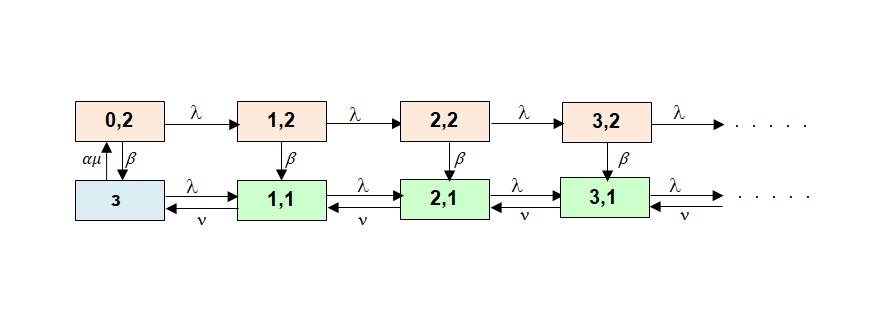
\includegraphics[width=\textwidth]{syst}\\
\\Множество состояний нашей системы можно разделить на три типа: первый - прибор включен и не находится в периоде задержки, в таком случае в системе находится количество заявок большее нуля. Состояния такого типа занумерованы на схеме выше $(1,1), (2,1), (3,1)$ и так далее, где первое число - это количество заявок в системе, а второе - единица, чтобы отметить этот тип состояний. \\
\\Второй тип - прибор выключен. Состояния такого типа занумерованы $(0,2), (1,2), (2, 2)$ и так далее, где первое число - это количество заявок в системе, а второе число - два. Если количество заявок $n$ в данном типе будет не равно нулю, то из состояния $(n, 2)$ второго типа система перейдет в состояние $(n, 1)$ первого типа сразу после включения прибора. Если система в состоянии $(0,2)$, то есть заявок в системе нет, и прибор выключен, то система может перейти в состояние $(1,2)$, если во время отключения придет одна заявка, или в состояние (з), период задержки, если прибор включится, но за время отключения ни одного требования так и не придет. \\
\\
Третий тип - прибор в режиме задержки. В этом случае заявок в системе не будет, период задержки может наступить после обслуживания последнего требования или после того, как прибор включился, но новых требований за время отключения не пришло. 
\\

\subsection{Вывод уравнений баланса}\\
Таким образом, состояние системы в момент $t$ описывается цепью Маркова $\Omega(t) = (q(t), \zeta(t))$, где $q(t)$ - число заявок на орбите, a $\zeta(t)$ определяется следующим образом: \\
\begin{equation*}
\zeta(t) =
\begin{cases}
1 &\text{прибор включен,}\\
2 &\text{прибор выключен,}\\
\text{з} &\text{прибор в периоде задержки.}
\end{cases}
\end{equation*}

Если система в момент времени $t$ находится в периоде задержки, то нет необходимости вводить переменную $q(t)$, ведь в этом случае в системе не будет ни одного требования. В этом случае естественно положить $\Omega(t) = \zeta(t)$.\\
\\Множество состояний цепи Маркова $\Omega(t)$ можно предстваить в виде $\Omega(t)=\{\text{з}, (0,2), (i,2), (i,1)\}$, где $i>0$.\\
\\Полученная цепь Маркова однородна: \\
$$\textbf{P}(t) = (P_{ij}(t)) = P(\Omega (s +t)=j\,|\, \Omega (s) =i) = Р(\Omega (t) = j\,|\, \Omega (0) = i).$$
Пусть $(P_{ij}(t))$ —матрица переходных вероятностей. Она удовлетворяет уравнению Колмогорова - Чепмена: \\
\\
$$\textbf{P}(t+s)=\textbf{P}(t)\textbf{P}(s). $$
По определению, инфинитезимальная матрица, $Q = \lim_{h \ti \infty} \dfrac{P(h) - E}{h} $, или, что эквивалентно $Q = (q_{ij}) = \left(\dfrac{dP_{ij}(h)}{dh}\right)\Big|_{h=0}$.\\
\\
Из уравнения Колмогорова - Чепмена следует прямое уравнение Колмогорова: 
$$ \dfrac{dP(t)}{dt} = P(t)Q.$$
Стационарное распределение цепи Маркова - это распределение вероятности, которое не меняется с течением времени: $\exists \lim\limits_{t \to \infty} P_{ij}(t) = P_j$. В частности $\lim\limits_{t \to \infty} \dfrac{dP_{ij}(t)}{dt} = 0 $ .\\
\\ 
Мы рассматриваем стационарный случай, прямое уравнение Колмогорова примет вид: 
$$\dfrac{dP(t)}{dt} = 0 =\textbf{P}(t)\textbf{Q}\, - \text{в матричной форме, или:}$$
$$ q_jP_j = \sum\limits_{k\neq j}P_kq_{kj}.$$ 
\\
На рисунке рядом со стрелками указаны $q_{ij}$ для нашей модели, то есть производные вероятностей перехода из состояния $i$ в состояние $j$ за малое время $h$. \\
\\
Уравнение для состояния $(1,1)$:
$$ (\lambda + \nu)\cdot P_{ij} = \lambda P_3 + \beta P_{12} +\nu P_{21}. \eqno(16)$$ 
\\
Уравнения для остальных состояний первого типа (состояния $(w, 1), \,\text{где}\, w = 1, 2, 3, ...)$: 
$$(\lambda+\nu)\cdot P_{w 1},l= \lambda P_{w-1 1} + \beta P_{w 2} +\nu P_{w+1 1}\eqno(17)$$\\
Уравнение для состояния $(0,2)$: 
$$(\lambda + \beta)\cdot P_{0 2} = \alpha\mu Р_3. \eqno(18) $$\\ 
Уравнения для остальных состояний второго типа (состояния (s, 1), где s = 2, 3, 4...): 
$$(\lambda +\beta) \cdot P_{s2} = \lambda P_{s-1 2}\qquad \text{где s= 1,2...} \eqno(19)$$\\
Уравнение для состояния (з): 
$$(\lambda+\alpha\mu)\cdot P_3=\beta P_{02}+\nu P{11} \eqno(20)$$ \\
Введем производящие функции: 
$$P_2 (z) = \sum\limits_{i=0}^\infty P_{i2}\cdot z^i, $$
$$P_1 (z) = \sum\limits_{i=1}^\infty P_{i1}\cdot z^{i-1}. $$
Так, домножая каждое из уравнений $(16), (18), (20)$ на $z^0$, а уравнения $(17), (19)$, на $z^1, z^2, z^3$ и так далее, мы получим систему: \\
\begin{equation*}
\begin{cases}
(\lambda +\beta)\cdot P_2 (z) = z\lambda P_2 (z) + \alpha \mu P_3,\\
(\lambda+\nu-\dfrac{\nu}{z}-\lambda z)\cdot P_1 (z) = \lambda P_3 + \dfrac{\beta}{z} P_2(z) -\dfrac{\beta}{z} P_{02} - \dfrac{\nu}{z} P_{11},\\
(\lambda + \alpha \mu)\cdot P_3 = \beta P_{02} + \nu P_{11}.
\end{cases}
\end{equation*}\\
Из первого уравнения системы можно выразить $P_2(z)$: 
$$P_2(z) = \dfrac{\alpha \mu P_3}{\beta + \lambda -\lambda z}  \eqno(21)$$
Тогда, подставляя $P_2 (z)$ во второе уравнение системы, получим: 
$$(\lambda+\nu-\dfrac{\nu}{z}-\lambda z)\cdot P_1 (z) - \lambda P_3 - \dfrac{\beta\alpha \mu P_3}{z(\beta + \lambda -\lambda z)} + \dfrac{\beta}{z} P_{02} + \dfrac{\nu}{z} P_{11} = 0\eqno(22)$$
Выразим $P_1 (z)$ и $P_2 (z)$ через $P_3$:  
\begin{equation*}
\begin{cases}
P_2 (z) = \dfrac{\alpha \mu P_3}{\beta + \lambda -\lambda z},\\
(\lambda-\dfrac{\nu}{z})(1-z)\cdot P_1 (z) =\dfrac{P_3 (1-z)(\lambda^2 z -\alpha \mu \lambda - \beta \lambda - \lambda^2)}{z(\beta + \lambda -\lambda z)},\\
(\lambda + \alpha \mu)\cdot P_3 = \beta P_{02} + \nu P_{11}.
\end{cases} \eqno(23)
\end{equation*}\\
Чтобы выразить $P_3$ воспользуемся нормировочным условием: 
$$P_1(1)+P_2(1)+P_3 = \sum\limits_{i=1}^\infty P_{i1}+  \sum\limits_{j=0}^\infty P_{j2} + P_3 = 1.$$
$$ \dfrac{P_3\cdot(-\alpha\mu\lambda -\beta\lambda)}{\beta(\nu - \lambda)} + \dfrac{\alpha\mu\cdotP_3}{\beta} + P_3 = 1. \eqno(24)$$
$$ P_3\cdot \dfrac{\nu(\alpha\mu+\beta)}{\beta(\nu - \lambda)}  = 1. \eqno(25)$$
Таким образом, получим $P_3$:
$$P_3 =\dfrac{\beta\left(1-\dfrac{\lambda}{\nu}\right)}{\alpha\mu+\beta}.\eqno(26) $$
\subsection{Необходимое и достаточное условие стабильности системы.}\\
Чтобы найти критерий стационарности, необходимо учесть: 
$$0< P_3 < 1;\,\,\, 0< P_{i1} < 1;\,\,\, 0 < P_{j2} < 1;\qquad \forall i > 0,\,\, \forall j \geqslant 0. $$
Каждый из параметров $\lambda, \nu, \mu, \beta, \alpha$ больше нуля. Очевидно, что знаменатель в дроби (26) больше числителя, поэтому правое неравенство верно всегда: 
$$ 0 < P_3 =\dfrac{\beta\left(1-\dfrac{\lambda}{\nu}\right)}{\alpha\mu+\beta} <1. \eqno(27)$$
Для того, чтобы выполнялось левое неравенство, необходимо: 
$$ \dfrac{\lambda}{\nu} < 1.\eqno(28)$$
Далее рассмотрим условия на параметры, возникающие при наложении аналогичных неравенств на вероятности вида $P_{i1}, P_{j2}, \forall i > 0, \forall j \geqslant 0$. Чтобы представить дробь в виде ряда, воспользуемся разложением вида: 
$$\dfrac{1}{1-z} = \sum\limits_{i=0}^{\infty}z^i, \text{где} z\in(-1;1). $$
$$ P_2(z)= \sum\limits_{i=0}^{\infty}P_{i2}\cdot z^i = \dfrac{\alpha \mu P_3}{\beta + \lambda -\lambda z}  =\dfrac{\alpha\mu\beta\left(1-\dfrac{\lambda}{\nu}\right)}{(\alpha\mu+\beta)(\beta+\lambda-\lambda z)}  =\dfrac{\alpha\mu\beta\left(1-\dfrac{\lambda}{\nu}\right)}{(\alpha\mu+\beta)(\beta+\lambda)}  \cdot \dfrac{1}{1-\dfrac{\lambda z}{\lambda +\beta}} = $$ 
$$=  \dfrac{\alpha\mu\beta\left(1-\dfrac{\lambda}{\nu}\right)}{(\alpha\mu+\beta)(\beta+\lambda)} \sum\limits_{i=0}^{\infty}\left(\dfrac{\lambda}{\lambda +\beta}\cdot z\right)^i.\eqno(29)$$\\
Таким образом, мы можем выразить $P_{i2},\quad \forall i \geqslant 0$:
$$P_{i2} = \dfrac{\alpha\mu\beta\left(1-\dfrac{\lambda}{\nu}\right)}{(\alpha\mu+\beta)(\beta+\lambda)}\cdot\left(\dfrac{\lambda}{\lambda +\beta}\right)^i.\eqno(30) $$\\
Аналогично представим в виде ряда $P_1(z)$:
$$ P_1(z) = \dfrac{P_3(\lambda^2+\alpha\mu\lambda+\beta\lambda-\lambda^2z)}{(\nu-\lambda z)(\lambda+\beta-\lambda z)} = \dfrac{P_3(\lambda^2+\alpha\mu\lambda+\beta\lambda-\lambda^2z)}{\nu(\lambda+\beta)\left(1-\dfrac{\lambda z}{\lambda + \beta}\right)\left(1-\dfrac{\lambda z}{\nu}\right)}= $$
$$= \dfrac{P_3(\lambda^2+\alpha\mu\lambda+\beta\lambda)}{\nu(\lambda+\beta)\left(1-\dfrac{\lambda z}{\lambda + \beta}\right)\left(1-\dfrac{\lambda z}{\nu}\right)}-\dfrac{P_3\lambda^2z}{\nu(\lambda+\beta)\left(1-\dfrac{\lambda z}{\lambda + \beta}\right)\left(1-\dfrac{\lambda z}{\nu}\right)} = $$ 
$$=\dfrac{P_3(\lambda^2+\alpha\mu\lambda+\beta\lambda)}{\nu(\lambda+\beta)}\cdot\dfrac{1}{\left(1-\dfrac{\lambda z}{\lambda + \beta}\right)\left(1-\dfrac{\lambda z}{\nu}\right)} - \dfrac{P_3\lambda^2}{\nu(\lambda+\beta)}\cdot\dfrac{z}{\left(1-\dfrac{\lambda z}{\lambda + \beta}\right)\left(1-\dfrac{\lambda z}{\nu}\right)}.$$\\
Разложим в ряд отдельно каждую дробь.
$$\dfrac{1}{\left(1-\dfrac{\lambda z}{\lambda + \beta}\right)\left(1-\dfrac{\lambda z}{\nu}\right)} = \dfrac{\lambda+\beta}{(\lambda + \beta -\nu)\left(1-\dfrac{\lambda z}{\nu}\right)}-  \dfrac{\nu}{(\lambda + \beta -\nu)\left(1-\dfrac{\lambda z}{\lambda+\beta}\right)}=$$
$$=\dfrac{\lambda+\beta}{\lambda+\beta-\nu}\sum\limits^\infty_{i=1}\left(\dfrac{\lambda}{\nu}\cdot z\right)^{i-1} - \dfrac{\nu}{\lambda+\beta-\nu}\sum\limits^\infty_{i=1}\left(\dfrac{\lambda}{\lambda+\beta}\cdot z\right)^{i-1}.$$
$$\dfrac{z}{\left(1-\dfrac{\lambda z}{\lambda + \beta}\right)\left(1-\dfrac{\lambda z}{\nu}\right)} = \dfrac{(\lambda+\beta)z}{(\lambda + \beta -\nu)\left(1-\dfrac{\lambda z}{\nu}\right)}-  \dfrac{\nu z}{(\lambda + \beta -\nu)\left(1-\dfrac{\lambda z}{\lambda+\beta}\right)}=$$
$$=\dfrac{\lambda+\beta}{\lambda+\beta-\nu}\sum\limits^\infty_{i=1}\left(\dfrac{\lambda}{\nu}\right)^{i-1}\cdot z^i - \dfrac{\nu}{\lambda+\beta-\nu}\sum\limits^\infty_{i=1}\left(\dfrac{\lambda}{\lambda+\beta}\right)^{i-1}\cdot z^{i-1}. $$
$$P_1(z) = \sum\limits_{i=1}^\infty P_{i1}z^{i-1} = \sum\limits^\infty_{i=1}\left( \left(\dfrac{\lambda}{\nu}\right)^{i}\cdot\dfrac{P_3(\lambda+\alpha\mu+\beta-\nu)}{\lambda+\beta-\nu} - \left(\dfrac{\lambda}{\lambda+\beta}\right)^{i}\cdot\dfrac{P_3\alpha\mu}{\lambda+\beta-\nu} \right)\cdot z^{i-1}.\eqno(31) $$
Таким образом, получаем $i>0$:
$$P_{i1}= \left(\dfrac{\lambda}{\nu}\right)^{i}\cdot\dfrac{P_3(\lambda+\alpha\mu+\beta-\nu)}{\lambda+\beta-\nu} - \left(\dfrac{\lambda}{\lambda+\beta}\right)^{i}\cdot\dfrac{P_3\alpha\mu}{\lambda+\beta-\nu}.\eqno(32)$$
Например, для $i=1$:
$$P_{11} = \dfrac{\lambda(\lambda+\alpha\mu+\beta)P_3}{\nu(\lambda+\beta)} = \dfrac{\lambda(\lambda+\alpha\mu+\beta)\beta\left(1-\dfrac{\lambda}{\nu}\right)}{\nu(\lambda+\beta)(\alpha\mu+\beta)}.\eqno(33)$$
\subsection{Операционные характеристики}
Мы нашли явный вид стационарного распределения: 
$$P_3 =\dfrac{\beta\left(1-\dfrac{\lambda}{\nu}\right)}{\alpha\mu+\beta}.\eqno(26) $$
$$P_{i2} = \dfrac{\alpha\mu\beta\left(1-\dfrac{\lambda}{\nu}\right)}{(\alpha\mu+\beta)(\beta+\lambda)}\cdot\left(\dfrac{\lambda}{\lambda +\beta}\right)^i, \quad\forall i\geqslant 0.\eqno(30) $$\\
$$P_{i1}= \left(\dfrac{\lambda}{\nu}\right)^{i}\cdot\dfrac{P_3(\lambda+\alpha\mu+\beta-\nu)}{\lambda+\beta-\nu} - \left(\dfrac{\lambda}{\lambda+\beta}\right)^{i}\cdot\dfrac{P_3\alpha\mu}{\lambda+\beta-\nu},\,\quad\forall i > 0.\eqno(32)$$
\\
Чтобы найденные решения системы действительно являлись стационарным распределением нужно, чтобы выполнялись неравенства: 
$$0< P_3 < 1;\,\,\, 0< P_{i1} < 1;\,\,\, 0 < P_{j2} < 1;\qquad \forall i > 0,\,\, \forall j \geqslant 0. $$
Каждое из неравенств будет выполнено при условии: 
$$ \dfrac{\lambda}{\nu} < 1.\eqno(28)$$
Найдем математическое ожидание числа требований в системе в стационарном случае: 
$$\mathbb{E}q=P_3\cdot 0+ \sum\limits_{i=1}^\infty P_{i1}\cdot i + \sum\limits_{j=0}^\infty P_{j2}\cdot j = $$
$$ \sum\limits_{i=1}^\infty \left( \left(\dfrac{\lambda}{\nu}\right)^{i}\cdot\dfrac{P_3(\lambda+\alpha\mu+\beta-\nu)}{\lambda+\beta-\nu} - \left(\dfrac{\lambda}{\lambda+\beta}\right)^{i}\cdot\dfrac{P_3\alpha\mu}{\lambda+\beta-\nu}  \right)\cdot i + \sum\limits_{j=0}^\infty \dfrac{\alpha\mu\beta\left(1-\dfrac{\lambda}{\nu}\right)}{(\alpha\mu+\beta)(\beta+\lambda)}\cdot\left(\dfrac{\lambda}{\lambda +\beta}\right)^j \cdot j.\eqno(34)$$
Воспользуемся разложением:
$$ \sum\limits_{n=0}^\infty n\cdot a^n = \dfrac{a}{(a-1)^2}\qquad\text{верно при}\,\,|a|<1.$$
$$ \sum\limits_{i=0}^\infty \left(\dfrac{\lambda}{\nu}\right)^i\cdot i = \dfrac{\lambda\nu}{(\lambda - \nu)^2}.$$
$$ \sum\limits_{i=0}^\infty \left(\dfrac{\lambda}{\lambda+\beta}\right)^i\cdot i = \dfrac{\lambda(\lambda+\beta)}{\beta^2}.$$
$$\mathbb{E}q =\left( \dfrac{\beta\left(1-\dfrac{\lambda}{\nu}\right)(\lambda+\alpha\mu+\beta-\nu)}{(\lambda+\beta-\nu)(\alpha\mu+\beta)}\right)\cdot\dfrac{\lambda\nu}{(\lambda - \nu)^2}-\left( \dfrac{\left(1-\dfrac{\lambda}{\nu}\right)\alpha\mu\beta}{(\lambda+\beta-\nu)(\alpha\mu+\beta)}\right)\cdot\dfrac{\lambda(\lambda+\beta)}{\beta^2}+ $$
$$\dfrac{\left(1-\dfrac{\lambda}{\nu}\right)\alpha\mu\beta}{(\lambda+\beta)(\alpha\mu+\beta)}\right)\cdot\dfrac{\lambda(\lambda+\beta)}{\beta^2} = \dfrac{\lambda\beta^2(\lambda+\alpha\mu+\beta-\nu)}{\beta(\lambda+\beta-\nu)(\alpha\mu+\beta)(\nu-\lambda)}-\dfrac{\lambda\alpha\mu(\nu-\lambda)^2}{\beta(\lambda+\beta-\nu)(\alpha\mu+\beta)(\nu-\lambda)}=$$
$$=\dfrac{\lambda\alpha\mu\beta+\lambda\alpha\mu\nu-\lambda^2\alpha\mu+\lambda\beta^2}{\beta(\alpha\mu+\beta)(\nu-\lambda)}.\eqno(35)$$
Далее найдем формулу для $\mathbb{E}q^z$, где $q$ -- число требований в системе.
$$\pi(z)=\mathbb{E}z^q = P_3\cdot z^0+ \sum\limits_{i=1}^\infty P_{i1}\cdot z^i + \sum\limits_{j=0}^\infty P_{j2}\cdot z^j = P_3\cdot z^0 + z\cdot\dfrac{P_3(\lambda^2+\alpha\mu\lambda+\beta\lambda-\lambda^2z)}{(\nu-\lambda z)(\lambda+\beta-\lambda z)}+\dfrac{\alpha\mu P_3}{\beta+\lambda - \lambda z}=$$
$$=\dfrac{(\alpha\mu\nu+\nu(\lambda+\beta-\lambda z))\beta\left(1-\dfrac{\lambda}{\nu}\right)}{(\alpha\mu+\beta)(\nu-\lambda z)(\beta+\lambda -\lambda z)}. \eqno(36)$$
Заметим, что формула выше получена для стационарного распределения, не зависящего от времени.\\
\\
Таким образом, можем сформулировать результат в виде теоремы:\\
\textbf{Теорема.}\\
Если $\lambda < \nu$,тогда $\exists \lim\limits_{t \to \infty} \mathbb{E}z^{q(t)} = \pi (z) = \dfrac{(\alpha\mu\nu+\nu(\lambda+\beta-\lambda z))\beta\left(1-\dfrac{\lambda}{\nu}\right)}{(\alpha\mu+\beta)(\nu-\lambda z)(\beta+\lambda -\lambda z)}.$\\
Неравенство $\dfrac{\lambda}{\nu}<1$ является необходимым и достаточным условием стабильности для нашего случая.


\section{Оптимизационная задача}
Вернемся к модели 1 и решим следующую оптимизационную задачу:\\
Пусть $C_1$ -- стоимость ожидания одним требованием в единицу времени.\\
$C_2$ -- стоимость невыполнения работы, штраф за единицу времени.\\
Тогда получим уравнение издержек:\\
$$\Phi(m)\Delta = C_1\mathbb{E}q\Delta+C_2\mathbb{P}_m\Delta $$
Необходимо минимизировать издержки за единицу времени $\Delta$, где $P_m$ -- вероятность, что прибор находится в режиме перерыва, в системе $m-1$ требований, и за время $\Delta$ приходит ещё одно требование, и перерыв обрывается.\\
$\mathbb{E}q$ -- математическое ожидание количества требований в системе.\\
$\hat{P(z)}=\dfrac{1}{\tilde{\eta}}\int\limits^\infty_0V(z,t)\,dt = \dfrac{1}{\tilde{\eta}}\sum\limits^{m-1}_{i=0} \dfrac{1}{\lambda + \nu}\left( \dfrac{\lambda z}{\lambda +\nu}\right)^j $ -- предельное распределение в системе, находящейся в режиме перерыва.\\
Вероятность того, что в перерыве $m-1$ заявка ожидает обслуживания равна: $\dfrac{1}{\tilde{\eta}}\dfrac{1}{\lambda + \nu}\left( \dfrac{\lambda z}{\lambda +\nu}\right)^{m-1} $.\\
Вероятность того, что за малое время $\Delta$ поступило хотя бы 1 требование: $\mathbb{P}(X(\Delta) > 0) = 1 - \mathbb{P}(X(\Delta) = 0) = 1 - e^{-\lambda \Delta} = 1 - (1 +\lambda \Delta + \dfrac{(\lambda \Delta)^2}{2!} + ...) = \lambda\Delta + \bar{\bar{o}}(\Delta^2)$.\\
Вероятность нахождения системы в режиме перерыва: $\hat{p} = \dfrac{\bar{\eta}}{\mathbb{E}\tau}$.\\
Тогда $P_m = \dfrac{1}{\mathbb{E}\tau}\dfrac{\lambda\Delta}{\lambda + \nu}\left( \dfrac{\lambda}{\lambda +\nu}\right)^{m-1} $, где $\mathbb{E}\tau = \dfrac{\lambda\bar{\eta}\left(1 -\dfrac{\lambda}{\mu}\right) + \dfrac{\lambda}{\mu} Y_1}{\lambda \left(1 -\dfrac{\lambda}{\mu} \right)}$. 
\\Получим $\Phi(m)$:\\
$$\Phi(m) =C_1\left(\dfrac{\lambda}{\nu}\cdot\left(1+\dfrac{\nu}{\mu-\lambda}\right)-\dfrac{m\left(\dfrac{\lambda}{\lambda+\nu}\right)^m}{1-\left(\dfrac{\lambda}{\lambda+\nu}\right)^m}\right)} +C_2\dfrac{\lambda \left(1 -\dfrac{\lambda}{\mu} \right)}{\lambda\bar{\eta}\left(1 -\dfrac{\lambda}{\mu}\right) + \dfrac{\lambda}{\mu} Y_1}\left( \dfrac{\lambda}{\lambda +\nu}\right)^{m}=$$
 $$ C_1\dfrac{\lambda}{\nu}\cdot\left(1+\dfrac{\nu}{\mu-\lambda}\right)-C_1 \dfrac{m\left(\dfrac{\lambda}{\lambda+\nu}\right)^m}{1-\left(\dfrac{\lambda}{\lambda+\nu}\right)^m}+  C_2\dfrac{\nu \left(1 -\dfrac{\lambda}{\mu} \right)}{  1-\left(\dfrac{\lambda}{\lambda+\nu}\right)^m}\right)   }\left( \dfrac{\lambda}{\lambda +\nu}\right)^{m} =   $$
$$  C_1\dfrac{\lambda}{\nu}\cdot\left(1+\dfrac{\nu}{\mu-\lambda}\right) + \dfrac{\left(\dfrac{\lambda}{\lambda+\nu}\right)^m}{1-\left(\dfrac{\lambda}{\lambda+\nu}\right)^m}\cdot \left(C_2 \nu \left(1 -\dfrac{\lambda}{\mu} \right)} - C_1 m \right).   $$
Мы хотим найти такое количество заявок $m$, при котором издержки будут минимальны, то есть то число заявок, при котором нужно выводить прибор из состояния перерыва и начинать обслуживание. Мы ищем оптимальное число $m$.
Пусть $\dfrac{\lambda}{\lambda+\nu} = a$, $\tilde{C_2} = C_2 \nu \left(1 -\dfrac{\lambda}{\mu} \right) $, тогда поиск минимума функции $\Phi(m)$ сводится к поиску минимума функции $\tilde{\Phi(m)}$:
 $$\tilde{\Phi}(m) = \dfrac{a^m}{1-a^m}\cdot\left(\tilde{C_2} - C_1m\right).$$
$0<a<1, \tilde{C_2}, C_1, m > 0,$ тогда $\tilde{\Phi}(m)$ убывающая функция, и стремится к нулю при $m \to \infty$. 
\\
Получаем, что издержки будут минимизированы в случае, когда перерыв не обрывается. И в таком случае 
$$ \Phi_{opt} =  C_1\dfrac{\lambda}{\nu}\cdot\left(1+\dfrac{\nu}{\mu-\lambda}\right).$$
\\
\\
\\
\\
\\
\\
\\
\\

\section{Литература}
$[1]$ --  Афанасьев Г.А. (2021) Система M/G/1 с перерывами в работе прибора и их задержками. \textit{Теория вероятностей и ее применения}, Том 66, Выпуск 1.\\
$[2]$ --  Levy, Y. and Yechiali, U. (1975) Utilizatio of Idle Time in an M/G/1 Queueing System. \textit{Management Science,} 22, 202-211.\\
$[3]$ -- Т.Л. Саати, Элементы теории массового обслуживания и её приложения, 2-е изд., Советское радио, М., 1971, 520 с. \\
$[4]$ --  Афанасьева Л.Г., Булинская Е.В. (1980) Случайные процессы в теории массового обслуживания и управления запасами. -- М.: Изд-во МГУ, 14-26.\\
$[5]$ -- Афанасьева Л.Г. (2007) Очерки исследования операций. -- М.: Изд-во МГУ, 117-160. \\
$[6]$ -- W. L. Smith, $"$Renewal theory and its ramifications$"$, J. Roy. Statist. Soc. Ser. B, 20:2 (1958), 243-302. \\
\end{document}

